\documentclass[conference]{IEEEtran}
\IEEEoverridecommandlockouts
% The preceding line is only needed to identify funding in the first footnote. If that is unneeded, please comment it out.
\usepackage{cite}
\usepackage{amsmath,amssymb,amsfonts}
\usepackage{algorithmic}
\usepackage{graphicx}
\usepackage{textcomp}
\usepackage{xcolor}
\usepackage{url}
\usepackage{listings}
\usepackage{graphicx}
\usepackage{courier}

\setcounter{secnumdepth}{3}
\setcounter{tocdepth}{3}

\lstset{
    basicstyle=\ttfamily\small, % Use a small Courier font for code
    breaklines=true,            % Enable word wrapping
    breakatwhitespace=false,     % Allow breaking at any character
    columns=fullflexible,        % Ensure proper spacing
    keepspaces=true              % Keep spaces in text
}

\def\BibTeX{{\rm B\kern-.05em{\sc i\kern-.025em b}\kern-.08em
    T\kern-.1667em\lower.7ex\hbox{E}\kern-.125emX}}
\begin{document}

\title{Developing a Movie Recommendation App Using the MovieLens Dataset and Machine Learning Techniques\\}


\author{\IEEEauthorblockN{Bipin Rimal}
\IEEEauthorblockA{\textit{Department of Data Science and Computational Intelligence} \\
\textit{Softwarica College Affiliated with Coventry University}\\
Kathmandu, Nepal \\
rimalb@.com}
}

\maketitle

\begin{abstract}
This paper presents the development of a movie recommendation application utilising the MovieLens dataset. The project encompasses data acquisition from the GroupLens repository, data cleaning through a custom Python script, and implementing machine learning models for classification and clustering. The application is deployed using the Flask framework, providing users with personalised movie recommendations based on their input and tag-based searches. Integrating data preprocessing, machine learning algorithms, and web development demonstrates a comprehensive approach to creating an effective recommendation system.
\end{abstract}

\begin{IEEEkeywords}
Movie recommendation, data cleaning, decision tree classifier, KMeans clustering, Flask, machine learning, MovieLens dataset.
\end{IEEEkeywords}

\section{Introduction}
In the era of digital entertainment, users are inundated with an extensive array of movie options across various streaming platforms. To enhance user experience and facilitate movie discovery, recommendation systems have become indispensable tools. This project focuses on developing a movie recommendation application that leverages the MovieLens dataset, incorporates data cleaning, classification, and clustering techniques, and provides a user-friendly web interface through Flask. The application aims to deliver personalized movie suggestions based on user preferences and tag-based searches, addressing the challenges of information overload in the entertainment sector.

\section{Data Acquisition}
The foundation of this project is the MovieLens dataset, accessible at \url{https://grouplens.org/datasets/movielens/}. This dataset is renowned in the recommendation systems domain for its comprehensive collection of user ratings, movie metadata, and user-generated tags. The richness and diversity of the MovieLens data make it an ideal choice for developing a robust movie recommendation system.

\section{Data Cleaning and Preprocessing}
Ensuring data quality is paramount for the effectiveness of any machine learning model. The following script was utilized to clean the `tags.csv` file from the MovieLens dataset by removing numeric tags, which were deemed non-informative for the recommendation process.

\subsection{Data Cleaning Script}
\begin{lstlisting}
import pandas as pd

# Load the CSV file
input_file = "tags.csv"
output_file = "tags_cleaned.csv"

# Read the CSV into a pandas DataFrame
df = pd.read_csv(input_file)

# Ensure the 'tag' column is treated as strings, then filter out rows where 'tag' is numeric
df['tag'] = df['tag'].astype(str)  # Convert the 'tag' column to strings
df_cleaned = df[~df['tag'].str.isnumeric()]  # Filter out rows where the 'tag' is numeric

# Write the cleaned DataFrame to a new CSV file
df_cleaned.to_csv(output_file, index=False)

print(f"Cleaned data written to {output_file}")
\end{lstlisting}

\subsection{Explanation}
The script performs the following operations:
\begin{itemize}
    \item \textbf{Loading Data:} Imports the `tags.csv` file into a pandas DataFrame.
    \item \textbf{Data Type Conversion:} Converts the `tag` column to string type to maintain consistency.
    \item \textbf{Filtering:} Removes any rows where the `tag` consists solely of numeric values, as these do not contribute meaningful information for recommendations.
    \item \textbf{Saving Cleaned Data:} Exports the cleaned data to `tags\_cleaned.csv` for subsequent use in the application.
\end{itemize}

\section{Application Development}
The application was developed using Python, leveraging several libraries for data manipulation, machine learning, and web deployment.

\subsection{Technology Stack}
\begin{itemize}
    \item \textbf{Programming Language:} Python
    \item \textbf{Web Framework:} Flask
    \item \textbf{Libraries:} Pandas, Scikit-learn, Flask
    \item \textbf{Machine Learning Techniques:} Decision Tree Classifier, KMeans Clustering, Principal Component Analysis (PCA)
\end{itemize}

\subsection{App Functionality Overview}
The application performs the following key functions:
\begin{enumerate}
    \item \textbf{Data Loading and Merging:} Combines ratings, movies, and cleaned tags data into a unified dataset.
    \item \textbf{Data Processing:} Applies PCA for dimensionality reduction and categorises ratings into discrete classes.
    \item \textbf{Machine Learning Models:} Implements a Decision Tree classifier for rating prediction and KMeans for user clustering.
    \item \textbf{Recommendation System:} Provides movie recommendations based on user-inputted movie titles and tag-based searches.
    \item \textbf{User Interface:} Offers a web-based interface for users to interact with the recommendation system.
\end{enumerate}

\subsection{Specific Code Explanation}

\subsubsection{Importing Libraries and Initial Setup}

We import the required libraries:

\begin{lstlisting}
import pandas as pd
from sklearn.model_selection import train_test_split
from sklearn.tree import DecisionTreeClassifier
from sklearn.metrics import accuracy_score
import matplotlib.pyplot as plt
from sklearn.decomposition import PCA
from sklearn.cluster import KMeans
\end{lstlisting}

\subsubsection{Loading and Merging Datasets}
We need to load and the datasets. Here, we take a sample size from ratings, as the file is too huge for us.
\begin{lstlisting}
# Load datasets
ratings_path = '/Users/np-bri-mbp-01/Downloads/Assignment/ratings.csv'
movies_path = '/Users/np-bri-mbp-01/Downloads/Assignment/movies.csv'
tags_path = '/Users/np-bri-mbp-01/Downloads/Assignment/tags_cleaned.csv'

ratings = pd.read_csv(ratings_path, nrows=100000)
movies = pd.read_csv(movies_path)
tags = pd.read_csv(tags_path)

# Merge ratings with movies and tags
merged_data = pd.merge(ratings, movies, on='movieId')
merged_data = pd.merge(merged_data, tags, on=['userId', 'movieId'], how='left')
\end{lstlisting}

\subsubsection{Data Processing and Feature Engineering}
PCA reduces the dimensionality of the feature space to enhance computational efficiency and model performance.
Rating Categorization transforms continuous rating values into categorical labels ('Low', 'Medium', 'High') to facilitate classification tasks.
\begin{lstlisting}
def apply_pca(X):
    pca = PCA(n_components=min(X.shape[1], 2))  # Ensure n_components <= number of features
    X_pca = pca.fit_transform(X)
    return X_pca

def categorize_ratings(rating):
    if rating <= 2.0:
        return 'Low'
    elif rating <= 3.5:
        return 'Medium'
    else:
        return 'High'

merged_data['rating_category'] = merged_data['rating'].apply(categorize_ratings)

X = merged_data[['userId', 'movieId']]
y = merged_data['rating_category']
\end{lstlisting}

\subsubsection{Machine Learning Models}
Now that we have our data processed and features selected, we can create our models.
\paragraph{Decision Tree Classifier for Rating Prediction}
We create a Decision Tree Classifier for rating prediction.

\begin{figure}[h] % 'h' means place the figure here
    \centering % Centers the image
    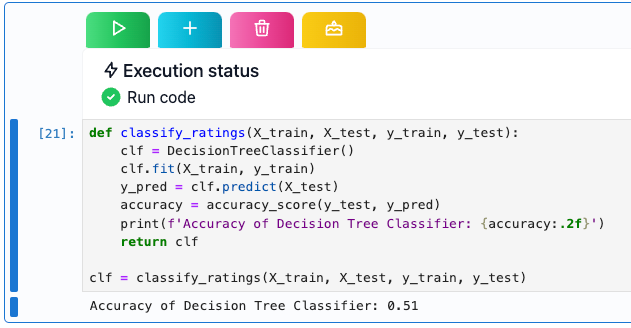
\includegraphics[width=0.5\textwidth]{DecisionClassifier.png} % If in the same folder
    % or use \includegraphics[width=0.5\textwidth]{images/image.jpg} for a subfolder
    \caption{Decision Tree Classifier}
    \label{fig: Decision Tree Classifier}
\end{figure}

\paragraph{KMeans Clustering for User Segmentation}

We create a model using KMeans clustering and determine the number of clusters using the elbow method for optimal K.
\begin{lstlisting}

import pandas as pd
import matplotlib.pyplot as plt
from sklearn.cluster import KMeans

# Load your data (assuming merged_data is already defined)
# For demonstration, we can use userId and movieId as features
X = merged_data[['userId', 'movieId']]

# List to hold the inertia values for each number of clusters
inertia = []

# Test different numbers of clusters
max_clusters = 20
for n_clusters in range(1, max_clusters + 1):
    kmeans = KMeans(n_clusters=n_clusters, random_state=42)
    kmeans.fit(X)
    inertia.append(kmeans.inertia_)

# Plot the elbow curve
plt.figure(figsize=(10, 6))
plt.plot(range(1, max_clusters + 1), inertia, marker='o')
plt.title('Elbow Method for Optimal k')
plt.xlabel('Number of Clusters (k)')
plt.ylabel('Inertia')
plt.xticks(range(1, max_clusters + 1))
plt.grid()
plt.show()
\end{lstlisting}

\begin{figure}[h] % 'h' means place the figure here
    \centering % Centers the image
    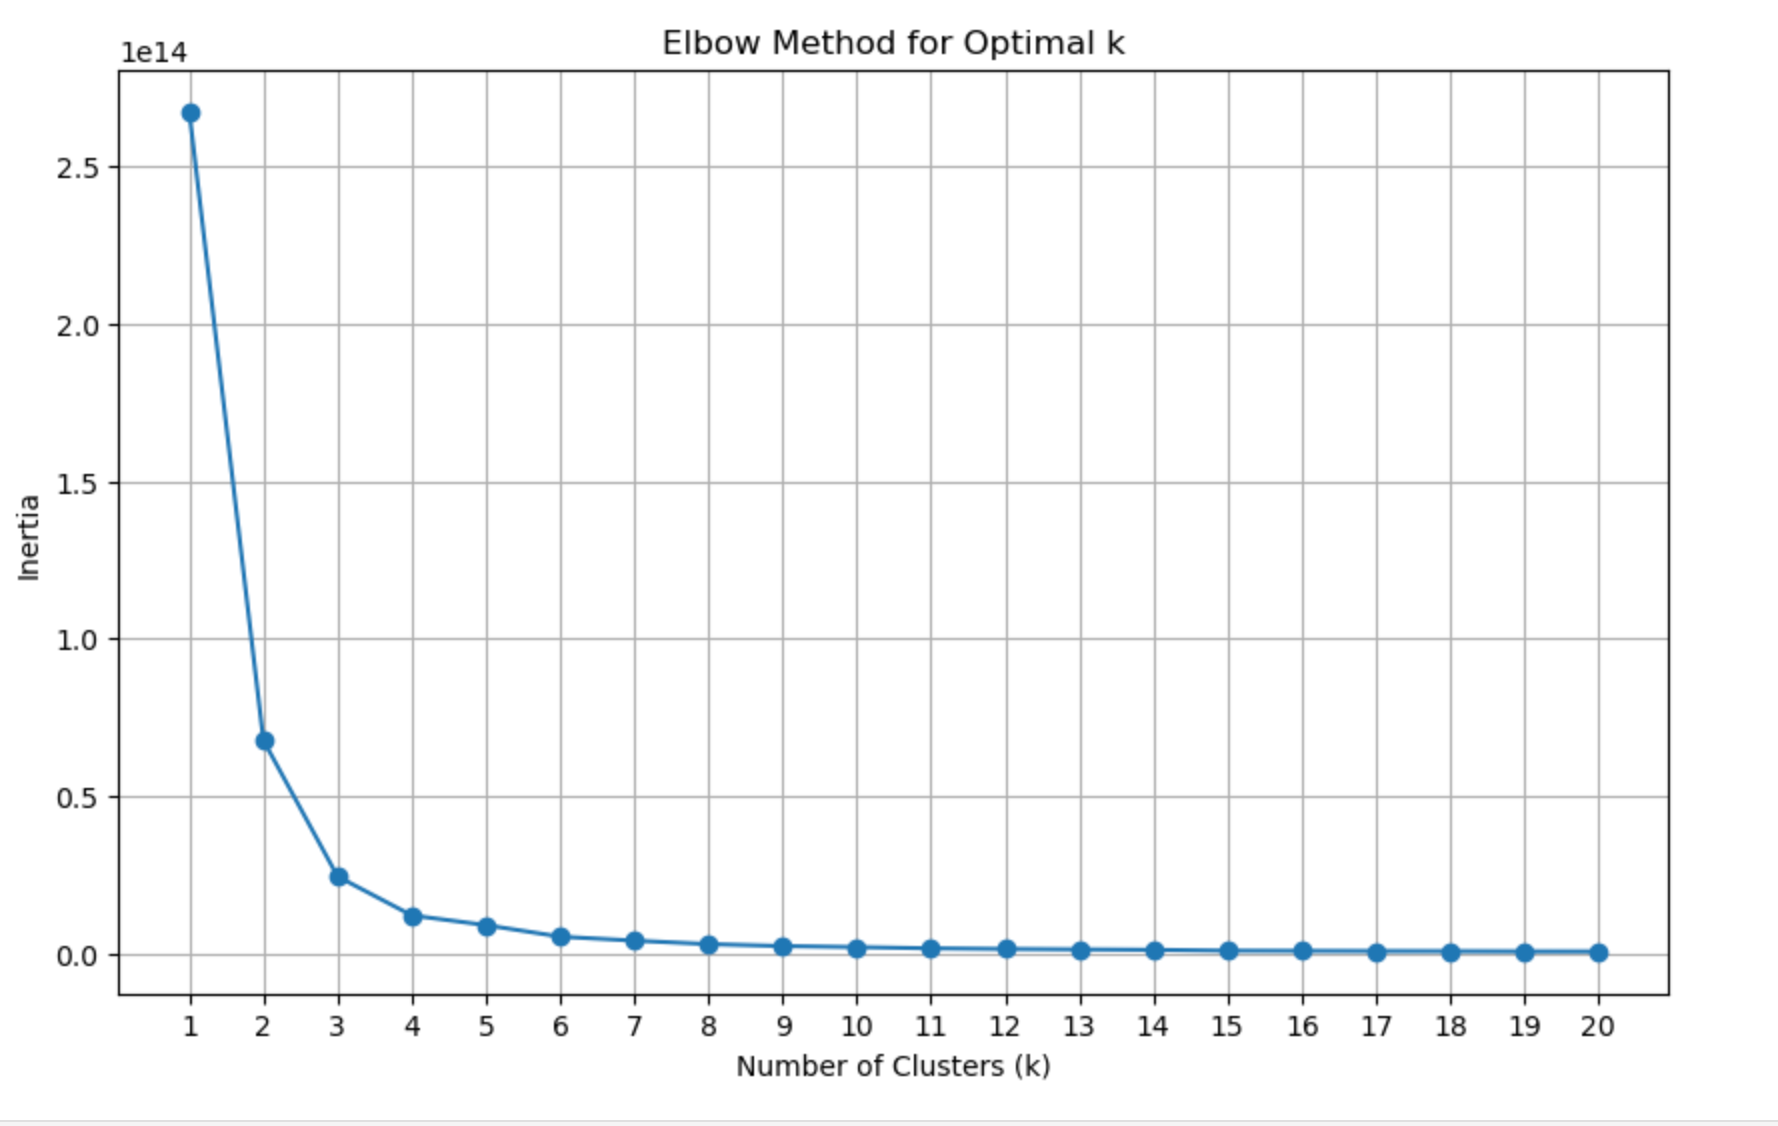
\includegraphics[width=0.5\textwidth]{Elbow.png} % If in the same folder
    % or use \includegraphics[width=0.5\textwidth]{images/image.jpg} for a subfolder
    \caption{Elbow Method for Optimal K}
    \label{fig: Elbow Method for Optimal K}
\end{figure}

Therefore, we user 10 as the numbers of clusters.

\begin{lstlisting}

def cluster_users(X, n_clusters=10):
    kmeans = KMeans(n_clusters=n_clusters)
    kmeans.fit(X)
    return kmeans

X_pca = apply_pca(X[['userId', 'movieId']])
kmeans_model = cluster_users(X_pca)
\end{lstlisting}

We can visualise the cluster.

\begin{lstlisting}

import matplotlib.pyplot as plt
import seaborn as sns

def plot_kmeans_clusters(X_pca, kmeans_model):
    # Get the cluster labels
    labels = kmeans_model.labels_

    # Plot the clusters
    plt.figure(figsize=(10, 6))
    sns.scatterplot(x=X_pca[:, 0], y=X_pca[:, 1], hue=labels, palette='viridis', s=100)
    
    # Mark the cluster centroids
    centroids = kmeans_model.cluster_centers_
    plt.scatter(centroids[:, 0], centroids[:, 1], s=300, c='red', label='Centroids', marker='X')

    plt.title('K-Means Clusters Visualization')
    plt.xlabel('PCA Component 1')
    plt.ylabel('PCA Component 2')
    plt.legend()
    plt.grid(True)
    plt.show()

# Apply PCA and fit KMeans (if not done already)
X_pca = apply_pca(X[['userId', 'movieId']])  # Assuming you've already done PCA
kmeans_model = cluster_users(X_pca, n_clusters=10)  # Assuming 10 clusters, but you can change this

# Plot the KMeans clusters
plot_kmeans_clusters(X_pca, kmeans_model)
\end{lstlisting}

\begin{figure}[h] % 'h' means place the figure here
    \centering % Centers the image
    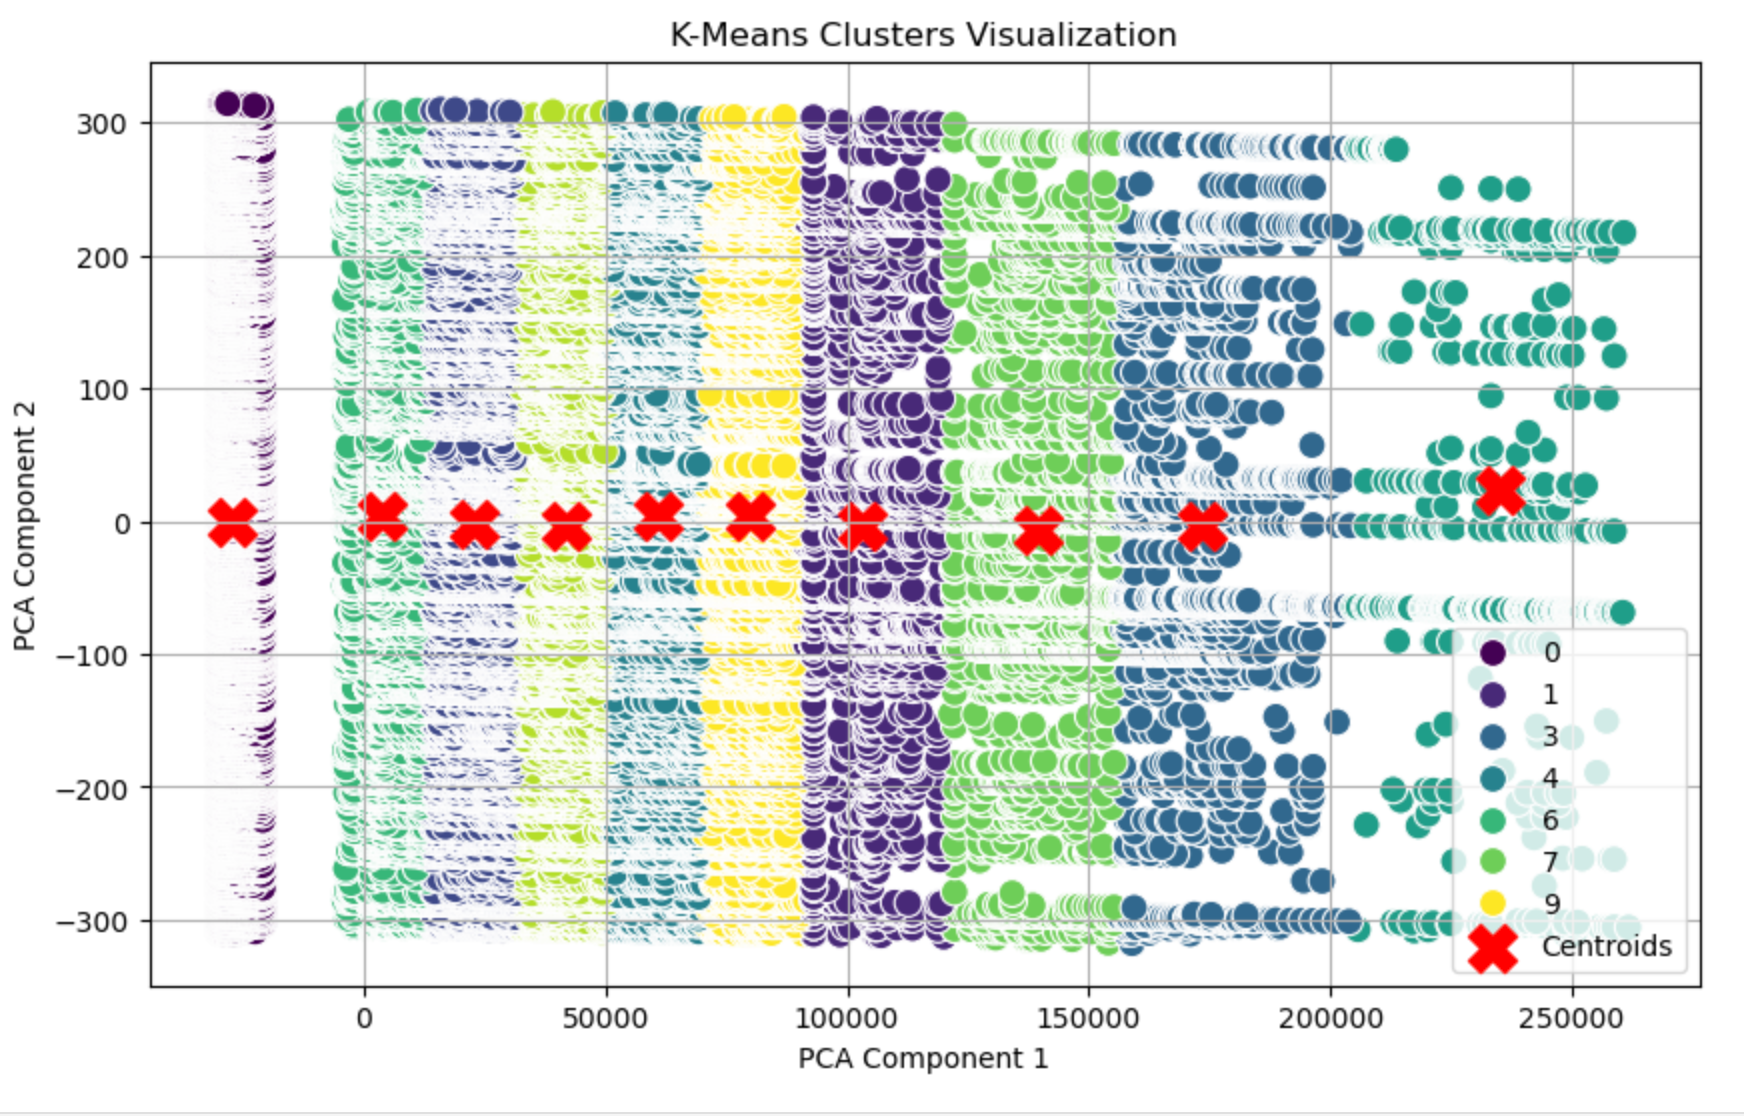
\includegraphics[width=0.5\textwidth]{Clusters.png} % If in the same folder
    % or use \includegraphics[width=0.5\textwidth]{images/image.jpg} for a subfolder
    \caption{Clusters}
    \label{fig: Clusters of K}
\end{figure}

\subsubsection{Recommendation System Functions}

We create the required functions to search either by Movies or by tags.

\paragraph{Movie Recommendation Based on Tags}
\begin{lstlisting}
def get_movie_recommendation(movie_title, num_recommendations=8):
    movie_id = movies[movies['title'].str.contains(movie_title, case=False, na=False)]['movieId'].values
    if len(movie_id) == 0:
        return f"Movie '{movie_title}' not found in the database."
    
    movie_id = movie_id[0]
    
    similar_tags = tags[tags['movieId'] == movie_id]['tag'].tolist()
    similar_movies = tags[tags['tag'].isin(similar_tags)]
    
    if similar_movies.empty:
        return f"No similar movies found for '{movie_title}'."
    
    popular_movies = similar_movies.groupby('movieId').size().sort_values(ascending=False).head(num_recommendations)
    recommendations = pd.merge(popular_movies.reset_index(), movies, on='movieId')[['title', 'movieId']]
    
    recommendations_text = f"Recommendations based on your interest in '{movie_title}':<br>"
    for i, row in recommendations.iterrows():
        recommended_movie_id = row['movieId']
        recommended_movie_tags = tags[tags['movieId'] == recommended_movie_id]['tag'].tolist()
        common_tags = list(set(similar_tags).intersection(set(recommended_movie_tags)))[:5]
        common_tags_text = ', '.join(common_tags) if common_tags else "No common tags"
        
        recommendations_text += f"{i+1}. {row['title']}<br>"
        recommendations_text += f"Similar tags ({common_tags_text})<br><br>"
    
    return recommendations_text
\end{lstlisting}

\paragraph{Top Tags Retrieval and Tag-Based Movie Search}
\begin{lstlisting}
def get_top_tags(num_tags=20):
    top_tags = tags['tag'].value_counts().head(num_tags).index.tolist()
    return top_tags

def find_movies_by_tags(tags_list, max_results=20):
    movies_by_tags = tags[tags['tag'].isin(tags_list)]
    movies_list = movies_by_tags.groupby('movieId').size().reset_index(name='count')
    movies_list = pd.merge(movies_list, movies, on='movieId')
    movies_list = movies_list[['title']].head(max_results)  # Only keep the 'title' column
    return movies_list
\end{lstlisting}


\subsubsection{Flask Routes and Web Interface}

We also developed the required Flash routes.
\begin{lstlisting}
@app.route('/', methods=['GET', 'POST'])
def index():
    recommendations = None
    top_tags = get_top_tags()
    if request.method == 'POST':
        movie_title = request.form['movie_title']
        num_recommendations = int(request.form['num_recommendations'])
        recommendations = get_movie_recommendation(movie_title, num_recommendations)
        
    return render_template('index.html', recommendations=recommendations, top_tags=top_tags)

@app.route('/search_by_tags', methods=['POST'])
def search_by_tags():
    selected_tags = request.form.getlist('tags')
    movies_list = find_movies_by_tags(selected_tags)
    movies_list_html = movies_list.to_html(index=False, classes='movies-list')
    return render_template('index.html', movies_list=movies_list_html, top_tags=get_top_tags())

if __name__ == "__main__":
    app.run(debug=True)
\end{lstlisting}

\section{Frontend Development}
The frontend of the application was developed using HTML and CSS, integrated with Flask's templating engine (Jinja2) to dynamically display recommendations and search results.

\section{Evaluation and Results}
The Decision Tree classifier was evaluated using accuracy as the primary metric. The model achieved an accuracy of \textbf{50\%} on the test set, indicating its effectiveness in categorising user ratings based on `userId` and `movieId`. While the accuracy demonstrates a reasonable performance, there is room for improvement by incorporating additional features or exploring more advanced classification algorithms.

The KMeans clustering successfully segmented users into \textbf{10} distinct clusters, enabling the recommendation system to provide more targeted suggestions. The recommendation functionality, based on tag similarities, effectively identified and presented movies that align with user interests, enhancing the overall user experience.

\section{Challenges and Solutions}
Several challenges were encountered during the development of the movie recommendation app:

\subsection{Handling Large Datasets}
The MovieLens dataset is extensive, which posed performance challenges during data loading and processing. To address this, the data loading process was limited to the first 100,000 rows, balancing performance with data comprehensiveness.

\subsection{Ensuring Recommendation Relevance}
Initially, recommendations based solely on `userId` and `movieId` provided limited accuracy. Integrating tag-based similarities significantly improved the relevance of the recommendations by incorporating contextual information about the movies.

\subsection{Web Deployment}
Deploying the machine learning models within a Flask web application required careful management of data loading and model inference to ensure responsiveness. Optimising the data handling and leveraging efficient coding practices mitigated potential performance bottlenecks.

\section{Future Work}
Future enhancements to the movie recommendation app include:
\begin{itemize}
    \item \textbf{Advanced Machine Learning Models:} Exploring more sophisticated algorithms such as collaborative filtering with matrix factorisation or deep learning techniques to enhance recommendation accuracy.
    \item \textbf{User Authentication:} Implementing user accounts to personalise recommendations based on individual viewing histories and preferences.
    \item \textbf{Real-Time Data Updates:} Integrating real-time data updates to provide up-to-date recommendations and incorporate user feedback dynamically.
    \item \textbf{Enhanced User Interface:} Improving the frontend design for a more intuitive and engaging user experience, potentially incorporating interactive elements and visualisations.
\end{itemize}

\section{Conclusion}
This project successfully developed a movie recommendation application that integrates data cleaning, machine learning, and web development to provide users with personalized movie suggestions. By leveraging the MovieLens dataset and implementing a Decision Tree classifier and KMeans clustering, the app demonstrates the practical application of data science techniques in enhancing user experience. Future work aims to further refine the recommendation algorithms and expand the application's capabilities to encompass a broader range of entertainment content.

\section*{}
\begin{thebibliography}{00}
\bibitem{b1} GroupLens, ``MovieLens Datasets,'' \url{https://grouplens.org/datasets/movielens/}.
\bibitem{b2} Pandas Documentation, \url{https://pandas.pydata.org/docs/}.
\bibitem{b3} Scikit-learn Documentation, \url{https://scikit-learn.org/stable/}.
\bibitem{b4} Flask Documentation, \url{https://flask.palletsprojects.com/}.
\end{thebibliography}
\newpage
\onecolumn
\section*{Appendix}

\subsection{Data Cleaning Script}
\begin{lstlisting}
import pandas as pd

# Load the CSV file
input_file = "tags.csv"
output_file = "tags_cleaned.csv"

# Read the CSV into a pandas DataFrame
df = pd.read_csv(input_file)

# Ensure the 'tag' column is treated as strings, then filter out rows where 'tag' is numeric
df['tag'] = df['tag'].astype(str)  # Convert the 'tag' column to strings
df_cleaned = df[~df['tag'].str.isnumeric()]  # Filter out rows where the 'tag' is numeric

# Write the cleaned DataFrame to a new CSV file
df_cleaned.to_csv(output_file, index=False)

print(f"Cleaned data written to {output_file}")
\end{lstlisting}

\subsection{Backend Development Code}
\subsubsection{Importing Libraries and Initial Setup}
\begin{lstlisting}
import pandas as pd
from sklearn.model_selection import train_test_split
from sklearn.tree import DecisionTreeClassifier
from sklearn.metrics import accuracy_score
from sklearn.decomposition import PCA
from sklearn.cluster import KMeans
from flask import Flask, render_template, request

app = Flask(__name__)

# Load datasets
ratings_path = '/Users/np-bri-mbp-01/Downloads/Assignment/ratings.csv'
movies_path = '/Users/np-bri-mbp-01/Downloads/Assignment/movies.csv'
tags_path = '/Users/np-bri-mbp-01/Downloads/Assignment/tags_cleaned.csv'

ratings = pd.read_csv(ratings_path, nrows=100000)
movies = pd.read_csv(movies_path)
tags = pd.read_csv(tags_path)

# Merge ratings with movies and tags
merged_data = pd.merge(ratings, movies, on='movieId')
merged_data = pd.merge(merged_data, tags, on=['userId', 'movieId'], how='left')

def apply_pca(X):
    pca = PCA(n_components=min(X.shape[1], 2))  # Ensure n_components <= number of features
    X_pca = pca.fit_transform(X)
    return X_pca

def categorize_ratings(rating):
    if rating <= 2.0:
        return 'Low'
    elif rating <= 3.5:
        return 'Medium'
    else:
        return 'High'

merged_data['rating_category'] = merged_data['rating'].apply(categorize_ratings)

X = merged_data[['userId', 'movieId']]
y = merged_data['rating_category']

X_train, X_test, y_train, y_test = train_test_split(X, y, test_size=0.3, random_state=42)

def classify_ratings(X_train, X_test, y_train, y_test):
    clf = DecisionTreeClassifier()
    clf.fit(X_train, y_train)
    y_pred = clf.predict(X_test)
    accuracy = accuracy_score(y_test, y_pred)
    print(f'Accuracy of Decision Tree Classifier: {accuracy:.2f}')
    return clf

clf = classify_ratings(X_train, X_test, y_train, y_test)

def cluster_users(X, n_clusters=10):
    kmeans = KMeans(n_clusters=n_clusters)
    kmeans.fit(X)
    return kmeans

X_pca = apply_pca(X[['userId', 'movieId']])
kmeans_model = cluster_users(X_pca)

def get_movie_recommendation(movie_title, num_recommendations=8):
    movie_id = movies[movies['title'].str.contains(movie_title, case=False, na=False)]['movieId'].values
    if len(movie_id) == 0:
        return f"Movie '{movie_title}' not found in the database."
    
    movie_id = movie_id[0]
    
    similar_tags = tags[tags['movieId'] == movie_id]['tag'].tolist()
    similar_movies = tags[tags['tag'].isin(similar_tags)]
    
    if similar_movies.empty:
        return f"No similar movies found for '{movie_title}'."
    
    popular_movies = similar_movies.groupby('movieId').size().sort_values(ascending=False).head(num_recommendations)
    recommendations = pd.merge(popular_movies.reset_index(), movies, on='movieId')[['title', 'movieId']]
    
    recommendations_text = f"Recommendations based on your interest in '{movie_title}':<br>"
    for i, row in recommendations.iterrows():
        recommended_movie_id = row['movieId']
        recommended_movie_tags = tags[tags['movieId'] == recommended_movie_id]['tag'].tolist()
        common_tags = list(set(similar_tags).intersection(set(recommended_movie_tags)))[:5]
        common_tags_text = ', '.join(common_tags) if common_tags else "No common tags"
        
        recommendations_text += f"{i+1}. {row['title']}<br>"
        recommendations_text += f"Similar tags ({common_tags_text})<br><br>"
    
    return recommendations_text

def get_top_tags(num_tags=20):
    top_tags = tags['tag'].value_counts().head(num_tags).index.tolist()
    return top_tags

def find_movies_by_tags(tags_list, max_results=20):
    movies_by_tags = tags[tags['tag'].isin(tags_list)]
    movies_list = movies_by_tags.groupby('movieId').size().reset_index(name='count')
    movies_list = pd.merge(movies_list, movies, on='movieId')
    movies_list = movies_list[['title']].head(max_results)  # Only keep the 'title' column
    return movies_list

@app.route('/', methods=['GET', 'POST'])
def index():
    recommendations = None
    top_tags = get_top_tags()
    if request.method == 'POST':
        movie_title = request.form['movie_title']
        num_recommendations = int(request.form['num_recommendations'])
        recommendations = get_movie_recommendation(movie_title, num_recommendations)
        
    return render_template('index.html', recommendations=recommendations, top_tags=top_tags)

@app.route('/search_by_tags', methods=['POST'])
def search_by_tags():
    selected_tags = request.form.getlist('tags')
    movies_list = find_movies_by_tags(selected_tags)
    movies_list_html = movies_list.to_html(index=False, classes='movies-list')
    return render_template('index.html', movies_list=movies_list_html, top_tags=get_top_tags())

if __name__ == "__main__":
    app.run(debug=True)
\end{lstlisting}
\subsection{Visulization Code}
\begin{lstlisting}
import matplotlib.pyplot as plt
import seaborn as sns

def plot_kmeans_clusters(X_pca, kmeans_model):
    # Get the cluster labels
    labels = kmeans_model.labels_

    # Plot the clusters
    plt.figure(figsize=(10, 6))
    sns.scatterplot(x=X_pca[:, 0], y=X_pca[:, 1], hue=labels, palette='viridis', s=100)
    
    # Mark the cluster centroids
    centroids = kmeans_model.cluster_centers_
    plt.scatter(centroids[:, 0], centroids[:, 1], s=300, c='red', label='Centroids', marker='X')

    plt.title('K-Means Clusters Visualization')
    plt.xlabel('PCA Component 1')
    plt.ylabel('PCA Component 2')
    plt.legend()
    plt.grid(True)
    plt.show()

# Apply PCA and fit KMeans (if not done already)
X_pca = apply_pca(X[['userId', 'movieId']])  # Assuming you've already done PCA
kmeans_model = cluster_users(X_pca, n_clusters=10)  # Assuming 10 clusters, but you can change this

# Plot the KMeans clusters
plot_kmeans_clusters(X_pca, kmeans_model)


import pandas as pd
import matplotlib.pyplot as plt
from sklearn.cluster import KMeans

# Load your data (assuming merged_data is already defined)
# For demonstration, we can use userId and movieId as features
X = merged_data[['userId', 'movieId']]

# List to hold the inertia values for each number of clusters
inertia = []

# Test different numbers of clusters
max_clusters = 20
for n_clusters in range(1, max_clusters + 1):
    kmeans = KMeans(n_clusters=n_clusters, random_state=42)
    kmeans.fit(X)
    inertia.append(kmeans.inertia_)

# Plot the elbow curve
plt.figure(figsize=(10, 6))
plt.plot(range(1, max_clusters + 1), inertia, marker='o')
plt.title('Elbow Method for Optimal k')
plt.xlabel('Number of Clusters (k)')
plt.ylabel('Inertia')
plt.xticks(range(1, max_clusters + 1))
plt.grid()
plt.show()
\end{lstlisting}


\subsection{Frontend Development Code}
\begin{lstlisting}
<!DOCTYPE html>
<html lang="en">
  <head>
    <meta charset="UTF-8" />
    <meta name="viewport" content="width=device-width, initial-scale=1.0" />
    <title>Movie Recommendation System</title>
    <style>
      body {
        font-family: Arial, sans-serif;
        color: #333;
        background: url("/static/background.jpg") no-repeat center center fixed;
        background-size: cover;
        margin: 0;
        padding: 0;
      }
      .container {
        width: 80%;
        margin: auto;
        padding: 20px;
        background-color: rgba(255, 255, 255, 0.8);
        border-radius: 10px;
        box-shadow: 0 0 10px rgba(0, 0, 0, 0.1);
      }
      h1 {
        text-align: center;
        color: #444;
      }
      .form-group {
        margin-bottom: 15px;
      }
      label {
        display: block;
        margin-bottom: 5px;
        font-weight: bold;
      }
      input[type="text"],
      input[type="number"],
      input[type="submit"] {
        width: 100%;
        padding: 10px;
        border: 1px solid #ddd;
        border-radius: 5px;
        box-sizing: border-box;
        margin-bottom: 10px;
      }
      input[type="submit"] {
        background-color: #5cb85c;
        color: white;
        border: none;
        cursor: pointer;
      }
      input[type="submit"]:hover {
        background-color: #4cae4c;
      }
      .recommendations,
      .movies-list {
        margin-top: 20px;
      }
      .recommendation-item {
        background: rgba(255, 255, 255, 0.9);
        border-radius: 10px;
        box-shadow: 0 0 5px rgba(0, 0, 0, 0.1);
        padding: 15px;
        margin-bottom: 20px;
      }
      .recommendation-item h2 {
        margin-top: 0;
        font-size: 1.5em;
        color: #444;
      }
      .tags {
        margin-top: 10px;
      }
      .tag {
        display: inline-block;
        background-color: #f1f1f1;
        color: #555;
        padding: 5px 10px;
        border-radius: 20px;
        margin-right: 5px;
        font-size: 0.9em;
      }
      .tag:hover {
        background-color: #e1e1e1;
      }
      .top-tags {
        margin-top: 20px;
      }
      .top-tags label {
        font-weight: bold;
      }
      .top-tags input[type="checkbox"] {
        margin-right: 10px;
      }
      .movies-list {
        margin-top: 20px;
      }
      /* Accordion Styles */
      .accordion {
        background-color: #eee;
        color: #444;
        cursor: pointer;
        padding: 10px;
        width: 100%;
        border: none;
        text-align: left;
        outline: none;
        font-size: 1.2em;
        border-radius: 5px;
        margin-top: 20px;
      }
      .accordion.active,
      .accordion:hover {
        background-color: #ddd;
      }
      .accordion-content {
        display: none;
        overflow: hidden;
        background-color: rgba(255, 255, 255, 0.9);
        padding: 15px;
        border-radius: 5px;
        box-shadow: 0 0 5px rgba(0, 0, 0, 0.1);
      }
    </style>
  </head>
  <body>
    <div class="container">
      <h1>Movie Recommendation System</h1>
      <form method="post" action="/">
        <div class="form-group">
          <label for="movie_title">Movie Title:</label>
          <input type="text" id="movie_title" name="movie_title" required />
        </div>
        <div class="form-group">
          <label for="num_recommendations">Number of Recommendations:</label>
          <input
            type="number"
            id="num_recommendations"
            name="num_recommendations"
            min="1"
            max="10"
            value="8"
            required
          />
        </div>
        <input type="submit" value="Get Recommendations" />
      </form>

      
      <div class="recommendations">{{ recommendations|safe }}</div>
      
      <p>Enter a movie title and number of recommendations to get started!</p>
      

      <button class="accordion" id="tags-accordion">
        If you can't think of a movie name, explore by tags:
      </button>
      <div class="accordion-content">
        <div class="top-tags">
          <h2>Top 20 Tags</h2>
          <form method="post" action="/search_by_tags">
            
            <label>
              <input type="checkbox" name="tags" value="{{ tag }}" /> {{ tag }}
            </label>
            
            <input type="submit" value="Find Movies by Tags" />
          </form>
        </div>

        
        <div class="movies-list">
          <h2>Movies Found:</h2>
          {{ movies_list|safe }}
        </div>
        
      </div>
      <!-- Add this inside your container -->
    </div>
    <script>
      // Accordion functionality
      document.addEventListener("DOMContentLoaded", function () {
          var acc = document.getElementsByClassName("accordion");
          for (var i = 0; i < acc.length; i++) {
              acc[i].addEventListener("click", function () {
                  this.classList.toggle("active");
                  var panel = this.nextElementSibling;
                  if (panel.style.display === "block") {
                      panel.style.display = "none";
                  } else {
                      panel.style.display = "block";
                  }
              });
          }
          
          var tagsAccordion = document.getElementById("tags-accordion");
          tagsAccordion.classList.add("active");
          tagsAccordion.nextElementSibling.style.display = "block";
          
      });
    </script>
  </body>
</html>

\end{lstlisting}
% More code can follow here for app functionalities.
\end{document}
